\documentclass[11pt,a4paper]{article}
\usepackage[lmargin=1in,rmargin=1in,tmargin=1in,bmargin=1in]{geometry}
\usepackage[pagewise]{lineno} %line numbering
\usepackage{setspace}
\usepackage{ulem} %strikethrough - do not \sout{\cite{}}
\usepackage{xcolor} %change font color
\usepackage{graphicx}
\usepackage{filecontents}
\usepackage{tablefootnote}
\usepackage{footnotehyper}
\usepackage{subfig}
\usepackage[yyyymmdd]{datetime} %date format
\renewcommand{\dateseparator}{.}
\graphicspath{{../img/}} %path to graphics
\setcounter{secnumdepth}{5} %set subsection to nth level
\usepackage{caption}
\captionsetup[table]{skip=11pt} %sets a space after table caption
\usepackage{times}
\usepackage{tabto} %general tabbed spacing
\usepackage{longtable} %need to put label at top under caption then \\ - use spacing
\usepackage[stable,hang,flushmargin]{footmisc} %footnotes in section titles and no indent
\usepackage[round]{natbib} %parenthesis instead of brackets for inline citations
\usepackage{enumitem}
\usepackage{boldline}
\usepackage{makecell}
\usepackage{booktabs}
\usepackage{amssymb}
\usepackage{amsmath}
\usepackage{physics}
\usepackage{tabularx}
\usepackage{multirow}
\usepackage{lscape}
\usepackage{array}
\usepackage{caption}
\usepackage[labelfont=bf]{caption}
\usepackage{chngcntr}
\usepackage{hyperref}

\newcommand{\edit}[1]{\textcolor{blue}{#1}} %shortcut for changing font color on revised text
\newcommand{\fn}[1]{\footnote{#1}} %shortcut for footnote tag
\newcommand*\sq{\mathbin{\vcenter{\hbox{\rule{.3ex}{.3ex}}}}} %makes a small square as a separator $\sq$
\renewcommand\labelenumi{(\theenumi)} %changes 1. to (1) in enumerated list

\usepackage{fancyhdr}
\pagestyle{fancy}
\fancyhf{} %move page number to bottom right
\renewcommand{\headrulewidth}{0.5pt} %turn off line in header
\lhead{\scriptsize \href{../ne450.html}{NE450 - Principles of nuclear engineering}}
\chead{\scriptsize \today}
\rhead{\scriptsize \href{3-nuclear-fuel-cycle-overview.html}{Project 3 - Nuclear fuel cycle overview}}
\rfoot{\thepage}

\begin{filecontents}{references.bib}
    @misc{
        ,
        author = {{}},
        title = {{}},
        year = {}
    }
    @article{
        ,
        author = {{}},
        journal = {},
        pages = {},
        title = {{}},
        volume = {},
        year = {}
    }
    @techreport{
        ,
        author = {{}},
        title = {{}},
        year = {},
        institution = {},
        number = {}
    }
\end{filecontents}

\begin{document}

\begin{titlepage}
    \title{
        NE450 - Principles of nuclear engineering\\
        Project 3 - Nuclear fuel cycle overview\\
    }
    \author{
        Name
        \\ \\ \\
        University of Idaho $\sq$ Idaho Falls Center for Higher Education
        \\ \\
        Engineering/Technology Management, Industrial Technology\\and\\Nuclear Engineering Department
        \\ \\ \\
        email 
    }
\clearpage %not have page number on title page
\maketitle
\vspace*{\fill}
\begin{flushright}{
        Total - 200
}
\end{flushright}
\thispagestyle{empty} %start with page number 1 on second page
\end{titlepage}

\section{Preface to the homework project}

\noindent Refer to these references to start for aqueous reprocessing -
\begin{enumerate}[leftmargin=*,topsep=0pt,font=\bfseries]
    \item\href{../homework-resources/countercurrent-equilibrium-extraction.pdf}{Countercurrent equilibrium extraction}
    \item\href{../homework-resources/nuclear-fuel-reprocessing.pdf}{Nuclear fuel reprocessing}
    \item\href{https://youtu.be/HGwHLaPhw30}{Liquid-liquid extraction example problem}
    \item\href{https://youtu.be/vK8XGYwnZv4}{Liquid-liquid extraction example problem}
    \item\href{../homework-resources/principles-stagewise-separation-process-calculations.pdf}{Principles of stagewise separation process calculations}
\end{enumerate}
\vspace{\baselineskip}

\noindent Use standard assumptions -
\begin{itemize}[leftmargin=*,topsep=0pt,font=\bfseries]
    \item Constant distribution coefficient
    \item Complete mixing
    \item Fresh solvent
\end{itemize}
\vspace{\baselineskip}

\noindent In problems 3 - 8, please address how the solution will affect the engineering design of a commercial scale PUREX facility. \textit{Required for full credit.}

\newpage

\begin{enumerate}[leftmargin=*,topsep=0pt,font=\bfseries]
    \item\textbf{}
        \vspace{0.25in}\\
    
        
        
        
        
        
        
        
        
        
        
        
        
        
        \newpage
    \item\textbf{(10) Based on this, derive the minimum and maximum scattered neutron energies.}
        \vspace{0.25in}\\
        
        
        
        
        
        
        
        
        
        
        
        
        
        
        \newpage
    \item\textbf{(10) Derive the average energy of the scattered neutron and the average energy loss.}
        \vspace{0.25in}\\

        
        
        
        
        
        
        
        
        
        
        
        
        
        \newpage
    \item\textbf{(10) Find the limit of $\alpha$ with increasing $A$. What are the implications?}
        \vspace{0.25in}\\

        
        
        
        
        
        
        
        
        
        
        
        
        
        \newpage
    \item\textbf{(10) Do the same for average fractional energy loss versus $\alpha$.}
        \vspace{0.25in}\\














        \newpage
    \item\textbf{(10) Based on this, what materials are more attractive for slowing down neutrons and why?}
        \vspace{0.25in}\\

        
        
        
        
        
        
        
        
        
        
        
        
        \newpage
    \item\textbf{(10) Plot $\xi$ versus $A$. What are the major observations and implications?}
        \vspace{0.25in}\\
        
        
        
        
        
        
        
        
        
        
        
        
        
        
        \newpage
    \item\textbf{(20) Derive $\xi$. Apply the definition of \href{https://courses.lumenlearning.com/uidaho-riskassessment/chapter/statistical-moments/}{expected value for a continuous random variable} and the probability distribution per unit energy loss. \textit{The probability distribution can just be looked up and not derived, but please explain the functional behavior.}}
        \vspace{0.25in}\\
        
        
        
        
        
        
        
        
        
        
        
        
        
        
        \newpage
    \item\textbf{(10) Plot the average number of collisions versus $A$ for a 2 MeV neutron slowing down to 0.025 eV, for water, boron, carbon, sodium, and uranium. Comment on the results.}
        \vspace{0.25in}\\
        
        
        
        
        
        
        
        
        
        
        
        
        
        
        \newpage
    \item\textbf{(10) Is an inelastic scattering endothermic or exothermic? Please explain why. Similarly, is radiative capture endothermic or exothermic? \textit{Show with math.}}
        \vspace{0.25in}\\
        
        
        
        
        
        
        
        
        
        
        
        
        
        
        \newpage
    \item\textbf{(15) Why is boron an attractive neutron capture material?}
        \vspace{0.25in}\\
        
        
        
        
        
        
        
        
        
        
        
        
        
        \newpage
    \item\textbf{(15) Compute and plot the mean free path for scattering and absorption versus mass for water, boron, carbon, sodium, and uranium and comment on the results. How does this compare to (9)?}
        \vspace{0.25in}\\
        
        
        
        
        
        
        
        
        
        
        
        
        
        
        \newpage
    \item\textbf{(10) Derive and compute the most probable energy and velocity for thermal ($1/v$) neutrons.}
        \vspace{0.25in}\\
        
        
        
        
        
        
        
        
        
        
        
        
        
        
        \newpage
    \item\textbf{(10) Derive and compute mean energy and velocity of thermal ($1/v$) neutrons.}
        \vspace{0.25in}\\
        
        
        
        
        
        
        
        
        
        
        
        
        \newpage
    \item\textbf{(30) Consider two Ar filled rooms of 10 m wide ($x$) by 20 m long ($y$). A neutron source is located at the midpoint of the eastern room. A concrete wall of $x$ thickness separates the two rooms. How thick should the wall be to reduce the flux at the detector on the far western wall to 1\%? What would be the thicknesses for a lead-lined, concrete wall? Roughly compare the costs for each shielding material by deriving a cost function. Consider only scattering and absorption. \textit{See Figures \ref{fig-concrete-wall} and \ref{fig-concrete-lead-wall}.}}
        \vspace{0.25in}\\
\end{enumerate}

\newpage

%\begin{figure}[h!]
%    \centering
%    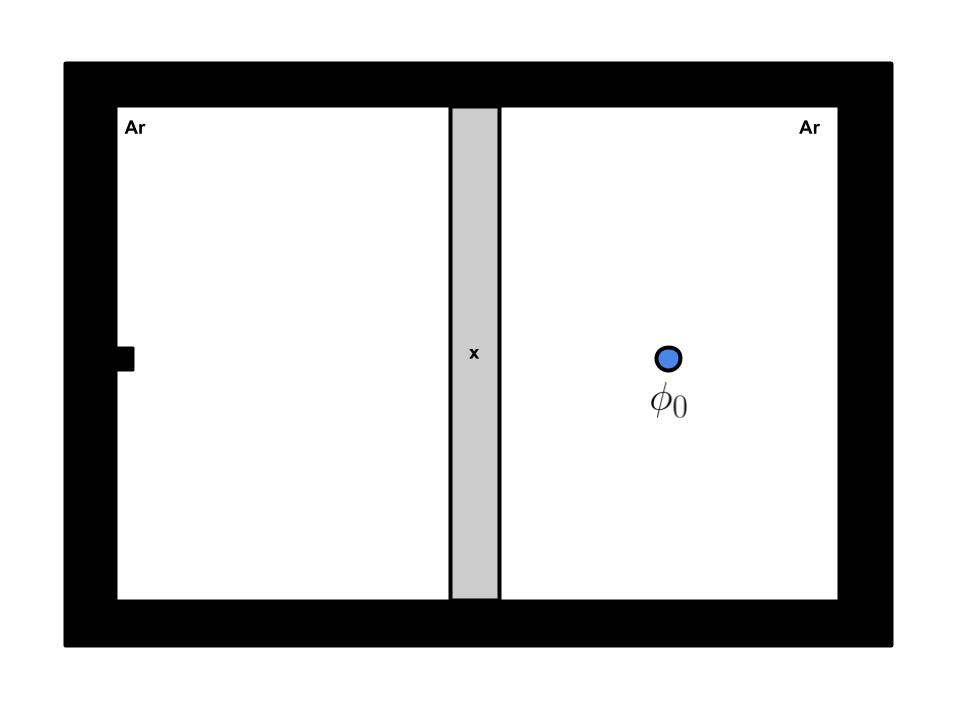
\includegraphics[width=0.75\textwidth]{hw2-15a.jpg}
%    \caption{Concrete wall}
%    \label{fig-concrete-wall}
%\end{figure}

%\begin{figure}[h!]
%    \centering
%    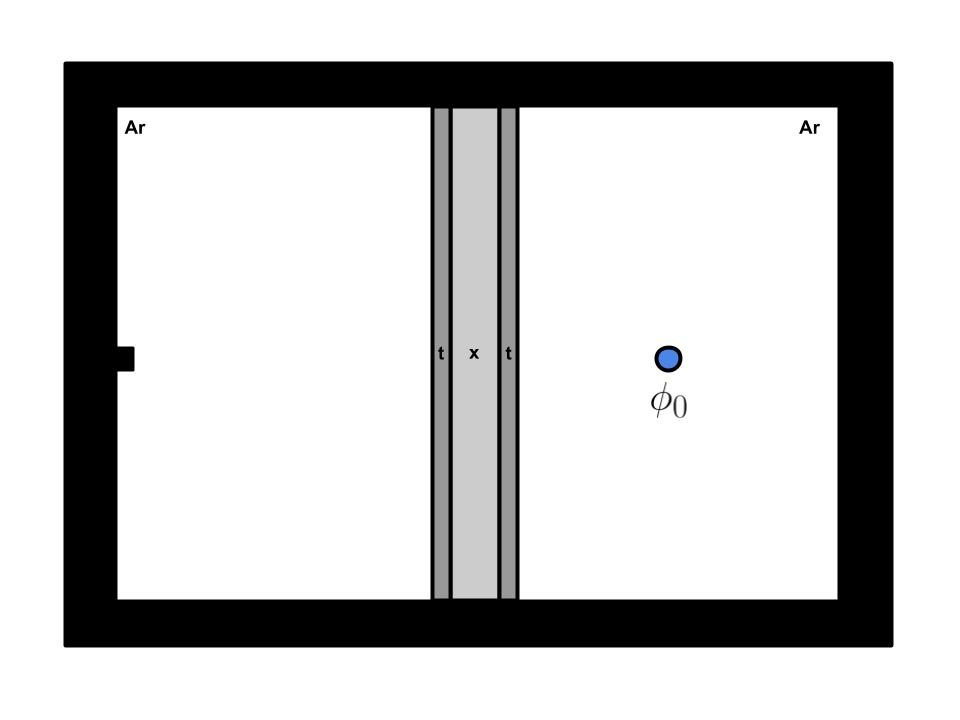
\includegraphics[width=0.75\textwidth]{hw2-15b.jpg}
%    \caption{Lead-lined concrete wall}
%    \label{fig-concrete-lead-wall}
%\end{figure}

\newpage 

\bibliographystyle{ieeetr}
\setlength{\bibhang}{0pt}
\bibliography{references}

\end{document}
